\section{Reverberation Chamber}
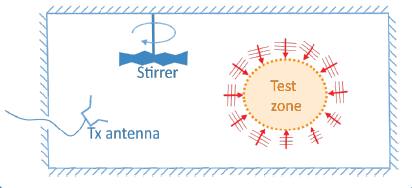
\includegraphics[width=8cm]{content/at_meas/pictures/reverberation_chamber}

A test chamber, contain ig a highly unsymmetric stirrer, designed to generate a \textbf{stochastical field distribution} in the test zone.

Ideally, it should have:
\begin{itemize}
  \item Electrically large cavity resonator with high $Q$ factor,
  \item High field strength for moderate input power,
  \item At least 60 resonant mode (IEEE 149--2022).
\end{itemize}

\subsection{Test Zone}
The ideal test zone field is:
\begin{itemize}
  \item isotropic (no preferred incident angle),
  \item homogenous (same magnitude everywhere),
  \item and unpolarized.
\end{itemize}

It can be described by a plane wave expansion:
\begin{equation}
  \bs{E}(\bs{r}) \oiint\limits_{\Omega} \bs{F}(\hat{\bs{k}}) \, e^{-j\bs{k}\cdot\bs{r}}\, \mathrm{d}^{2}\hat{\bs{k}}.
\end{equation}

\begin{enumerate}
  \item Bias correct
        \begin{equation*}
          \langle{|S_{21}|}^{2}\rangle \to \langle{|\tilde{S}_{21}|}^{2}\rangle = \langle{|S_{21} - \langle S_{21}\rangle|}^{2}\rangle
        \end{equation*}
  \item Basis equation for efficiency measurements
        \begin{align*}
          &\dfrac{{\langle b\rangle}^{2}}{a^{2}} = \langle {|S_{21}|}^{2} \rangle = \dfrac{Q}{16 \pi^{2}} \dfrac{\lambda^{3}}{V} \eta_{\text{RX}}^{\text{tot}} \, \eta_{\text{TX}}^{\text{tot}}\\
          &Q = \omega \tau : \quad \text{quality factor}\\
          &V : \quad \text{Chamber volume}
        \end{align*}
\end{enumerate}
